\newpage
\begin{section}{Arch Linux}
	\begin{subsection}{Mantainance}
		\begin{minted}{sh}
			#check file size
			du -sh .cache/
			#remove a file
			rm -rt .cache/
			#delete what you don't need in .config file
		\end{minted}

		specific mantainance:

		\begin{minted}{sh}
			#check the failed systems
			systemctl --failed
			#check the systemd journal
			sudo journalctl -p 3-xb
			#if the system doesn't boots then ctrl+alt+shift then timeshift -restore
			#then update mirrors
			#clar chache

			#then to update the whole system use:
			sudo pacman -Syyu
			#to check system updates
			sudo pacman -Syu
			#if you wan't to remove all packages in the drive use
			sudo pacman -Scc
			#remove all unwanted dependencies
			paru -Yc 
			#remove orphan packages
			sudo pacman -Rns \$(pacman - Qdtq)
			#sudo pacman -Syyy Syncrhonise data use "mirror1"
		\end{minted}

	\end{subsection}
	\begin{subsection}{Print in arch linux}

		install packages: usbutils, lsusb, cups

		use this to make cups usable
		\begin{minted}{sh}
			sudo systemct enable cups
			sudo systemctl start cups
			localhost:631

			lp -d HP_Officejey_Pro_8600]
		\end{minted}

	\end{subsection}


	\begin{subsection}{configure date and time}

		\begin{minted}{sh}
			hwclock --set --date = "04/32/2021 19:00:00"
			hwclock -hctosys
		\end{minted}

	\end{subsection}

	\begin{subsection}{Configure wireless}

		\begin{minted}{sh}
			#when entering an iso
			iwctl
			#then in the ui

			#to list all available devices
			device list

			#to scan networks
			station <device> scan

			#to get newworks
			station <device> get-network

			#to connect to a network
			station <device> connect "<name of network>"

			#to check if the connection is staable
			ping -c s 8.8.8.8

			#don't forget before rebooting the iso run
			pacman nmtui
		\end{minted}
		from Arch Water Linux
		\begin{minted}{sh}
			# to acces the gui for the internet
			nmtui
			# solve temporary failure in name resolution
			# change the /etc/resolve.conf file to nameserver 8.8.8.8

			# restart the resolved daemon
			sudo systemctl restart systemd-resolved.service
			# check that the daemon is running and active
			sudo systemctl status systemd-resolved.service
		\end{minted}

		dwm basic configuration
		\begin{minted}{sh}
			#MODKEY + shift + q to restart X server
			startx # to start the X server
		\end{minted}

	\end{subsection}
	\begin{subsection}{mount devices}
		mount usb sticks:
		\begin{minted}{sh}
			#to mount a usb stick
			mount /dev/sdb1 /mnt/<destination folder>
			#to unmount a sub stick
			umount /dev/sdb1
		\end{minted}
		mount an android device:
		\begin{minted}{sh}
			#to mount and android device
			simple-mtpfs --device 1 tablet/

			#to unmount an android device
			fusermount -u /tablet

		\end{minted}
	\end{subsection}
	\newpage
	\begin{subsection}{import export passwords from pass}
		export passwords:
		\begin{minted}{sh}
			# to list first the gpg keys
			gpg --list-secret-keys --keyid-format LONG
		\end{minted}
		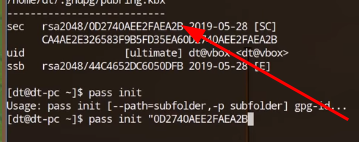
\includegraphics{img_ArchLinux/publicKeyImage.png}\caption{public key}
		\begin{minted}{sh}
			# to create the export files
			# save this files in a usb and use it later
			gpg --output MY_FILENAME_public.gpg --armor --export GPG_PUB_KEY
			gpg --output MY_FILENAME_secret.gpg --armor --export-secret-key GPG_PUB_KEY
			# in other pc import the gpg keys
			gpg --import MY_FILENAME_pub.gpg
			gpg --allow-secret-key-import --import MY_FILENAME_sec.gpg
			# now copy the .password-store folder from the main machine and paste it into the new machine
		\end{minted}


	\end{subsection}

\end{section}
